\section{Simulation Validation}
\label{sec:validation}

All three approximations were validated against discrete-event simulation of the
two-queue fork-join system.
Each scenario used 20\,M jobs with a 500\,K-job warmup period, repeated over
5 independent random seeds; the reported $\Tsim$ is the grand mean and the
95\% confidence interval is computed via the $t$-distribution across seeds
($\mathrm{df}=4$).
Results for $\Tul$~\eqref{eq:tul} and $\Tlh$~\eqref{eq:tlh} (with $\beta = 10$)
are shown in Table~\ref{tab:results} alongside the theoretical bounds.
Table~\ref{tab:results-lhe} compares $\Tlh$ and the enhanced approximation
$\Tlhe$~\eqref{eq:tlhe}.

\begin{table}[ht]
\centering
\caption{Approximations vs.\ simulation for heterogeneous two-queue fork-join.
         $\Tsim$ is the grand mean over 5 seeds; $\pm$ is the 95\% CI half-width.
         Errors are $(T_{\text{approx}} - \Tsim)/\Tsim \times 100\%$.}
\label{tab:results}
\resizebox{\textwidth}{!}{%
\begin{tabular}{@{}ccccccccccc@{}}
\toprule
$\mu_1$ & $\mu_2$ & $\lambda$ & $\rho_2$ & $\Tbot$
        & $\Tsim$ & $\pm$95\%\,CI & $\Tul$ & Err & $\Tlh$ & Err \\
\midrule
1.0 & 1.0 & 0.3 & 0.30 & 1.429 & 2.089 & 0.001 & 2.089 & $0.00\%$ & 2.089 & $0.00\%$ \\
1.0 & 1.0 & 0.6 & 0.60 & 2.500 & 3.562 & 0.004 & 3.562 & $+0.01\%$ & 3.562 & $+0.01\%$ \\
1.0 & 1.0 & 0.9 & 0.90 & 10.000 & 13.892 & 0.082 & 13.875 & $-0.12\%$ & 13.875 & $-0.12\%$ \\
\midrule
1.0 & 1.5 & 0.3 & 0.20 & 1.429 & 1.707 & 0.001 & 1.716 & $+0.57\%$ & 1.698 & $-0.51\%$ \\
1.0 & 1.5 & 0.6 & 0.40 & 2.500 & 2.768 & 0.003 & 2.799 & $+1.13\%$ & 2.776 & $+0.31\%$ \\
1.0 & 1.5 & 0.9 & 0.60 & 10.000 & 10.142 & 0.083 & 10.193 & $+0.50\%$ & 10.325 & $+1.80\%$ \\
\midrule
1.0 & 2.0 & 0.3 & 0.15 & 1.429 & 1.583 & 0.001 & 1.590 & $+0.44\%$ & 1.595 & $+0.75\%$ \\
1.0 & 2.0 & 0.6 & 0.30 & 2.500 & 2.624 & 0.003 & 2.641 & $+0.64\%$ & 2.667 & $+1.64\%$ \\
1.0 & 2.0 & 0.9 & 0.45 & 10.000 & 10.050 & 0.083 & 10.063 & $+0.12\%$ & 10.170 & $+1.19\%$ \\
\midrule
1.0 & 3.0 & 0.6 & 0.20 & 2.500 & 2.548 & 0.003 & 2.554 & $+0.22\%$ & 2.583 & $+1.39\%$ \\
1.0 & 5.0 & 0.6 & 0.12 & 2.500 & 2.516 & 0.003 & 2.517 & $+0.04\%$ & 2.533 & $+0.68\%$ \\
\bottomrule
\end{tabular}%
}
\end{table}

\paragraph{Homogeneous case ($\mu_1 = \mu_2 = 1.0$).}
Both approximations recover the Nelson--Tantawi formula~\eqref{eq:nelson-tantawi}
by construction; residual errors ($\leq 0.12\%$) are simulation noise.
At $\lambda = 0.9$ the CI half-width is $\pm 0.082$, reflecting the heavy-tailed
response-time distribution near saturation; the analytical value $13.875$ lies
well within this interval.

\paragraph{Moderate heterogeneity ($r = 1.5$).}
$\Tul$ shows consistent positive errors ($+0.50\%$ to $+1.13\%$) across all
loads.
$\Tlh$ is more accurate at low and moderate load, but reaches $+1.80\%$ at
heavy load ($\rho_2 = 0.6$).
The wider CIs at $\lambda = 0.9$ (half-width $\pm 0.083$) indicate substantial
variance in the heavy-load regime; a short-run single-seed estimate is biased
low near saturation, illustrating the
importance of long runs and multiple seeds in this regime.

\paragraph{High heterogeneity ($r \geq 2$).}
$\Tul$ errors fall below $0.64\%$ and improve further as $r$ increases
($\leq 0.04\%$ at $r = 5$).
$\Tlh$ errors are slightly larger (up to $+1.64\%$ at $r = 2$).
CIs are tight at low-to-moderate load ($\leq \pm 0.003$ for $\rho_2 \leq 0.45$)
and widen to $\pm 0.083$ near saturation ($\lambda = 0.9$); relative to
$\Tsim \approx 10$ this is still below $1\%$, confirming that 20\,M jobs over
5 seeds provide well-converged estimates in this regime.
As $r \to \infty$, both approximations converge to $\Tbot$.

Figure~\ref{fig:vs-load} plots the two approximations, bounds, and simulation
as functions of load for $\mu_1 = 1.0$, $\mu_2 = 2.0$.
Both $\Tul$ and $\Tlh$ track the simulation closely across the full load
range, lying between the theoretical bounds.
Figure~\ref{fig:vs-hetero} shows the same quantities as a function of
the heterogeneity ratio $\mu_2/\mu_1$ at fixed $\lambda = 0.6$.
Near homogeneity ($r \approx 1$), $\Tlh$ is more accurate; for $r \geq 3$,
$\Tul$ is slightly tighter.

\begin{figure}[ht]
\centering
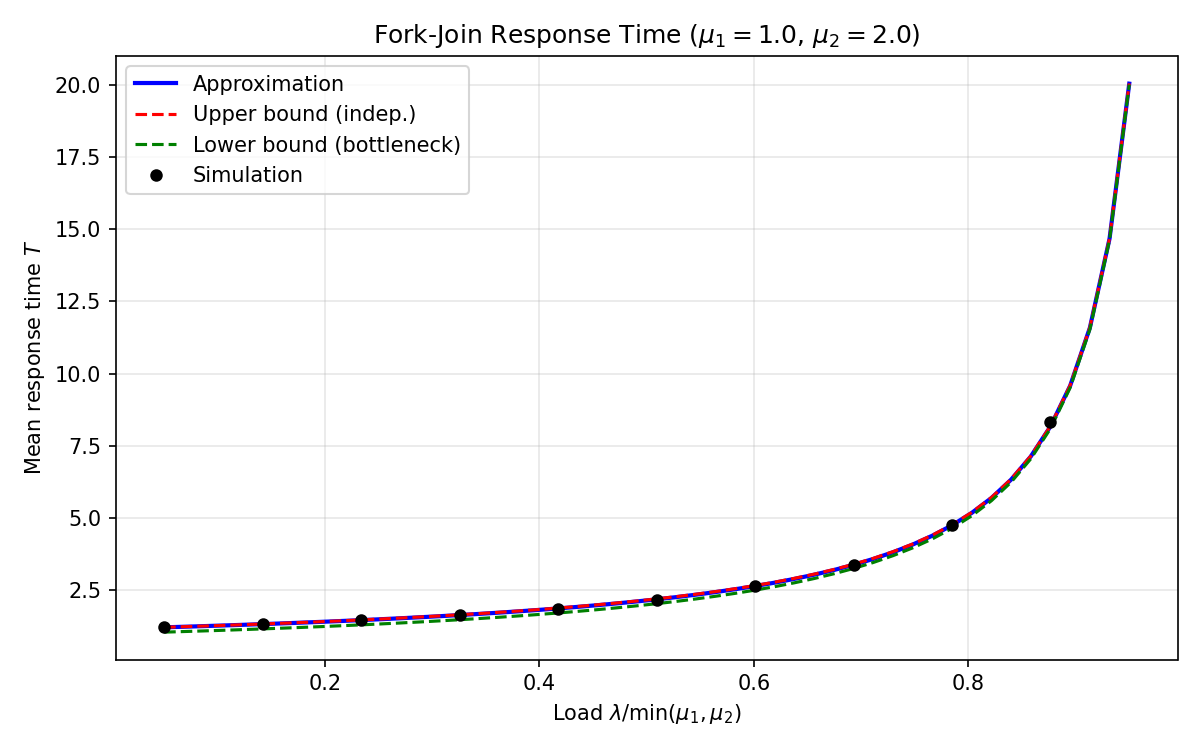
\includegraphics[width=0.85\textwidth]{figures/response_time_vs_load.png}
\caption{Mean response time vs.\ load $\lambda/\mumin$ for $\mu_1 = 1.0$,
         $\mu_2 = 2.0$.
         Markers: simulation. Lines: approximations and bounds.}
\label{fig:vs-load}
\end{figure}

\begin{figure}[ht]
\centering
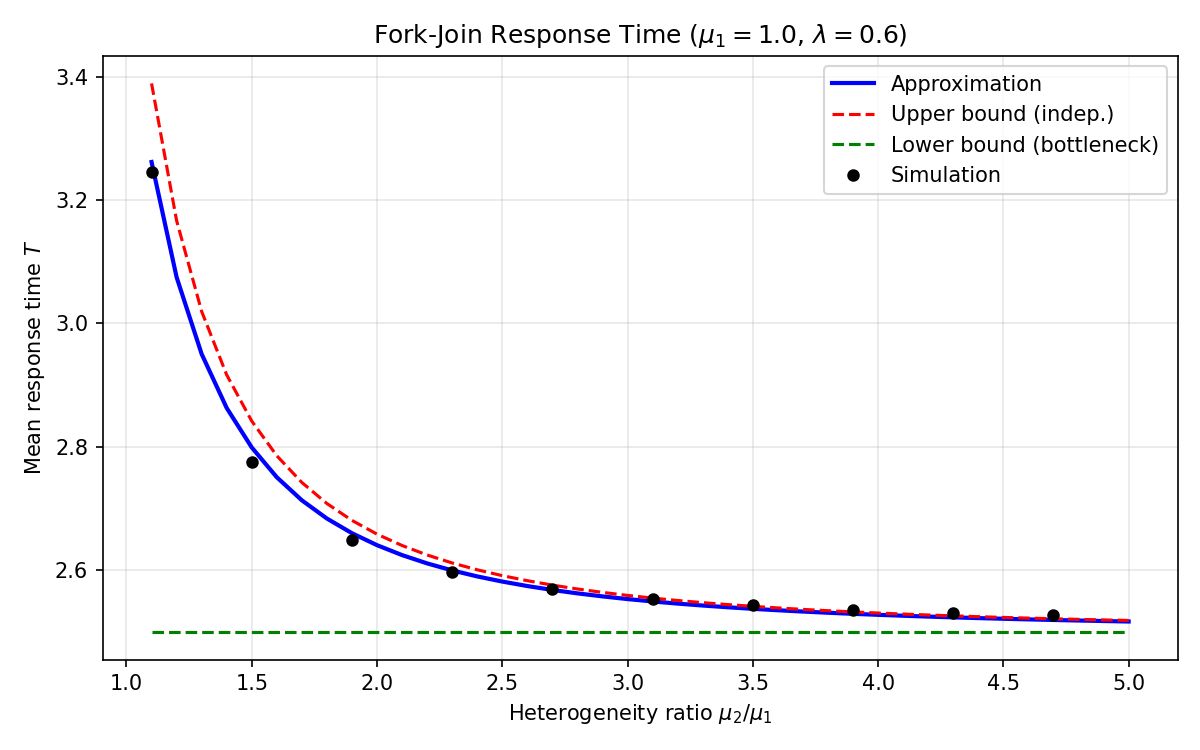
\includegraphics[width=0.85\textwidth]{figures/response_time_vs_heterogeneity.png}
\caption{Mean response time vs.\ heterogeneity ratio $\mu_2/\mu_1$ for
         $\mu_1 = 1.0$, $\lambda = 0.6$.
         Markers: simulation. Lines: approximations and bounds.}
\label{fig:vs-hetero}
\end{figure}

\subsection*{Sensitivity of $\Tul$ to Heterogeneity and Load}

Among the three approximations, $\Tul$ achieves the best uniform accuracy across
all loads and heterogeneity ratios, remains within the theoretical bounds by
construction, and requires no tunable parameters.
To characterize how its accuracy depends on both dimensions simultaneously,
we sweep the heterogeneity ratio $r = \mu_2/\mu_1$ from 1 to 8 across four
load levels chosen with a geometric spacing in the slack to saturation,
$1 - \rho \in \{0.48, 0.24, 0.12, 0.06\}$, i.e.\ $\rho \in \{0.52, 0.76, 0.88, 0.94\}$.

The heterogeneity grid uses 8 values $r \in \{1, 1.15, 1.3, 1.5, 2, 3, 5, 8\}$,
spaced more densely near $r = 1$ where $T$ transitions most steeply from
the homogeneous value to the bottleneck asymptote.
Each of the 32 simulation points uses 10\,M jobs with a 500\,K-job warmup
and a single random seed; 95\% confidence intervals are computed by the
normal approximation.

Figure~\ref{fig:tul-hetero-panel} shows the results.
At all four load levels, $\Tul$ closely tracks the simulation.
Most of the descent from the homogeneous value to the bottleneck plateau occurs
in $r \in [1, 2]$; beyond $r \approx 3$ the curves are essentially flat.
The relative error (right axis) peaks near $r = 1.15$--$1.3$ and is bounded
below $1.3\%$ for $\rho \leq 0.88$, consistent with the worst-case error of
$+1.13\%$ reported in Table~\ref{tab:results}.
At the highest load ($\rho = 0.94$), the single-seed estimate at $r = 1$
lies slightly above the exact homogeneous value, a reminder that estimates near
saturation require either multiple seeds or substantially longer runs to
eliminate transient bias; the displayed CI underestimates the true uncertainty
in this regime because consecutive response times are highly correlated near
saturation.

\begin{figure}[!ht]
\centering
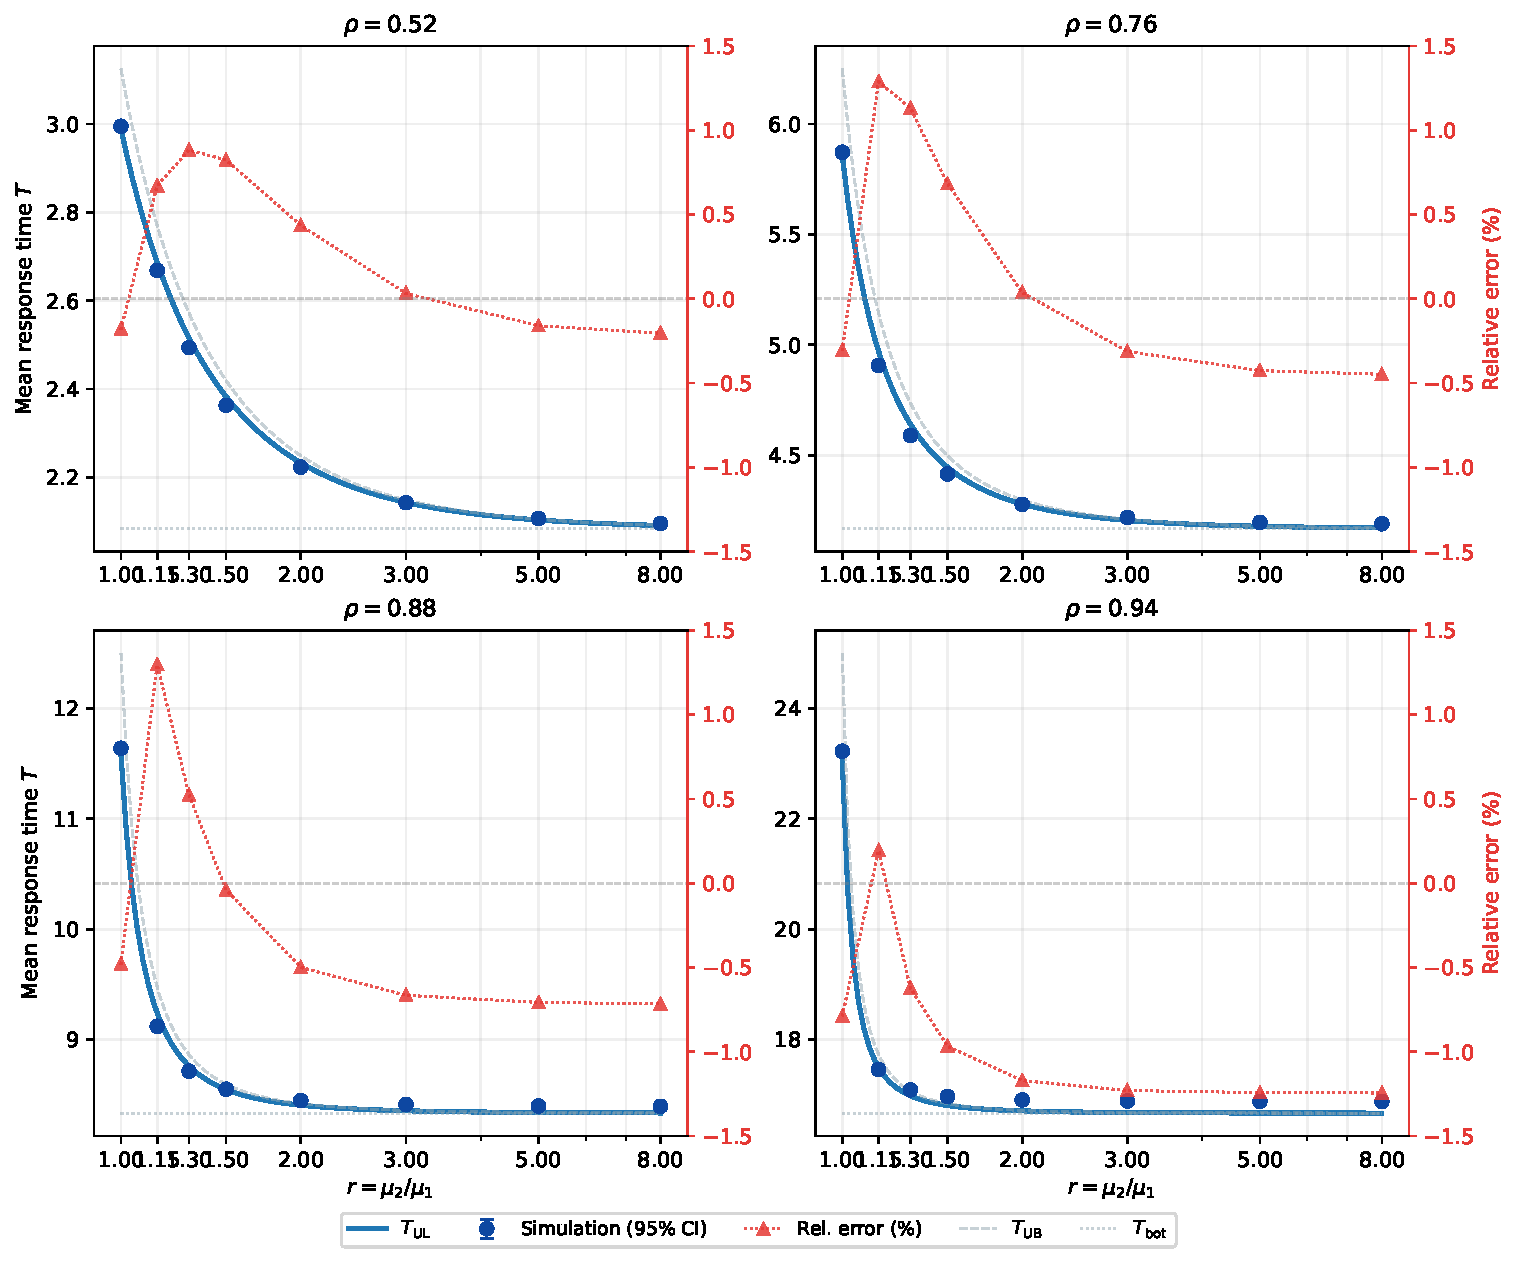
\includegraphics[width=\textwidth]{figures/t_ul_vs_heterogeneity.pdf}
\caption{$\Tul$ vs.\ heterogeneity ratio $r = \mumax/\mumin$ for four load
         levels $\rho \in \{0.52, 0.76, 0.88, 0.94\}$.
         Solid blue line: $\Tul$ (analytical); filled circles: simulation
         with 95\,\% CI bars ($10\,\mathrm{M}$ jobs, seed\,=\,42).
         Dashed and dotted gray lines: upper bound $\Tub$ and lower bound
         $\Tbot$.
         Right axis (red triangles): relative error
         $(\Tul - \Tsim)/\Tsim \times 100\%$.}
\label{fig:tul-hetero-panel}
\end{figure}

\subsection*{Enhanced LH Approximation}

Table~\ref{tab:results-lhe} compares $\Tlh$ and $\Tlhe$ against simulation.
Both use $\beta = 10$.

\begin{table}[ht]
\centering
\caption{$\Tlh$ vs.\ $\Tlhe$ vs.\ simulation for heterogeneous two-queue fork-join.
         $\Tsim$ and 95\% CI as in Table~\ref{tab:results}.
         Errors are $(T_{\text{approx}} - \Tsim)/\Tsim \times 100\%$.}
\label{tab:results-lhe}
\resizebox{\textwidth}{!}{%
\begin{tabular}{@{}cccccccccc@{}}
\toprule
$\mu_1$ & $\mu_2$ & $\lambda$ & $\rho_1$
        & $\Tsim$ & $\pm$95\%\,CI & $\Tlh$ & Err & $\Tlhe$ & Err \\
\midrule
1.0 & 1.0 & 0.3 & 0.30 & 2.089 & 0.001 & 2.089 & $0.00\%$ & 2.089 & $0.00\%$ \\
1.0 & 1.0 & 0.6 & 0.60 & 3.562 & 0.004 & 3.562 & $+0.01\%$ & 3.562 & $+0.01\%$ \\
1.0 & 1.0 & 0.9 & 0.90 & 13.892 & 0.082 & 13.875 & $-0.12\%$ & 13.875 & $-0.12\%$ \\
\midrule
1.0 & 1.5 & 0.3 & 0.30 & 1.707 & 0.001 & 1.698 & $-0.51\%$ & 1.710 & $+0.21\%$ \\
1.0 & 1.5 & 0.6 & 0.60 & 2.768 & 0.003 & 2.776 & $+0.31\%$ & 2.801 & $+1.20\%$ \\
1.0 & 1.5 & 0.9 & 0.90 & 10.142 & 0.083 & 10.325 & $+1.80\%$ & 10.362 & $+2.17\%$ \\
\midrule
1.0 & 2.0 & 0.3 & 0.30 & 1.583 & 0.001 & 1.595 & $+0.75\%$ & 1.589 & $+0.34\%$ \\
1.0 & 2.0 & 0.6 & 0.60 & 2.624 & 0.003 & 2.667 & $+1.64\%$ & 2.654 & $+1.14\%$ \\
1.0 & 2.0 & 0.9 & 0.90 & 10.050 & 0.083 & 10.170 & $+1.19\%$ & 10.150 & $+0.99\%$ \\
\midrule
1.0 & 3.0 & 0.6 & 0.60 & 2.548 & 0.003 & 2.583 & $+1.39\%$ & 2.561 & $+0.51\%$ \\
1.0 & 5.0 & 0.6 & 0.60 & 2.516 & 0.003 & 2.533 & $+0.68\%$ & 2.519 & $+0.13\%$ \\
\bottomrule
\end{tabular}%
}
\end{table}

\paragraph{Homogeneous case ($\mu_1 = \mu_2 = 1.0$).}
As proved in Section~\ref{sec:approx-lhe}, the quadratic coefficient $c_2 = 0$
when $r = 1$, so $\Tlhe \equiv \Tlh$.
Both recover Nelson--Tantawi exactly; residual errors ($\leq 0.12\%$) are
simulation noise.

\paragraph{Moderate heterogeneity ($r = 1.5$).}
$\Tlhe$ is slightly less accurate than $\Tlh$ across all loads
(worst case $+2.17\%$ vs.\ $+1.80\%$ at heavy load).
This regime is where the power-law model $h(r) = 1 + \tfrac{3}{8}r^{-\beta}$
is least reliable: $h(r)$ varies steeply near $r = 1$, and the resulting
systematic error in the heavy-traffic anchor dominates the benefit of
matching the first derivative.
Both LH variants are therefore less accurate than $\Tul$ ($+0.50\%$) in
this regime.

\paragraph{High heterogeneity ($r \geq 2$).}
$\Tlhe$ consistently outperforms $\Tlh$:
at $r = 2$ and $\lambda \in \{0.3, 0.6\}$ errors fall from $+0.75\%,\,+1.64\%$
to $+0.34\%,\,+1.14\%$; at $r = 3$ from $+1.39\%$ to $+0.51\%$;
and at $r = 5$ from $+0.68\%$ to $+0.13\%$.
In this regime $h(r) \approx 1$ and the first light-traffic derivative
$T_0'$ carries meaningful information about the service-time
heterogeneity that improves accuracy over a wide load range.
